\section{Results}
\label{sec:results}

\subsection{Steering Efficiency}
\label{sec:efficiency}

\Tabref{tab:efficiency} presents the peak steering efficiency for each intervention space. The residual stream achieves the highest efficiency at every operating point, producing $2.6\times$ more sentiment shift per unit of KL divergence than the MLP intermediate space.

\begin{table}[t]
\centering
\caption{Steering efficiency across intervention spaces. Efficiency is defined as sentiment probability shift per unit of KL divergence ($\eta = \Delta_{\text{sent}} / \KL$). The residual stream is $2.6\times$ more efficient than the MLP intermediate space at their respective optimal $\alpha$ values.}
\label{tab:efficiency}
\begin{tabular}{@{}lccc@{}}
\toprule
Space & Best Efficiency ($\eta$) & Optimal $\alpha$ & Max $\Delta_{\text{sent}}$ \\
\midrule
\residstream & {\bf 0.0130} & 10 & {\bf +0.000665} \\
\mlpout & 0.0062 & 10 & +0.000248 \\
\mlpinter & 0.0048 & 5 & +0.000243 \\
\bottomrule
\end{tabular}
\end{table}

All three spaces exhibit an inverted-U relationship between steering strength and effectiveness (\Figref{fig:efficiency}): sentiment shift increases at moderate $\alpha$ values, peaks, and then reverses at high $\alpha$ ($> 100$--$200$) as the intervention pushes activations out of the model's learned distribution. The MLP intermediate space reaches its peak at a lower $\alpha$ (5 vs.\ 10), consistent with its greater sensitivity to perturbation.

\begin{figure}[t]
\centering
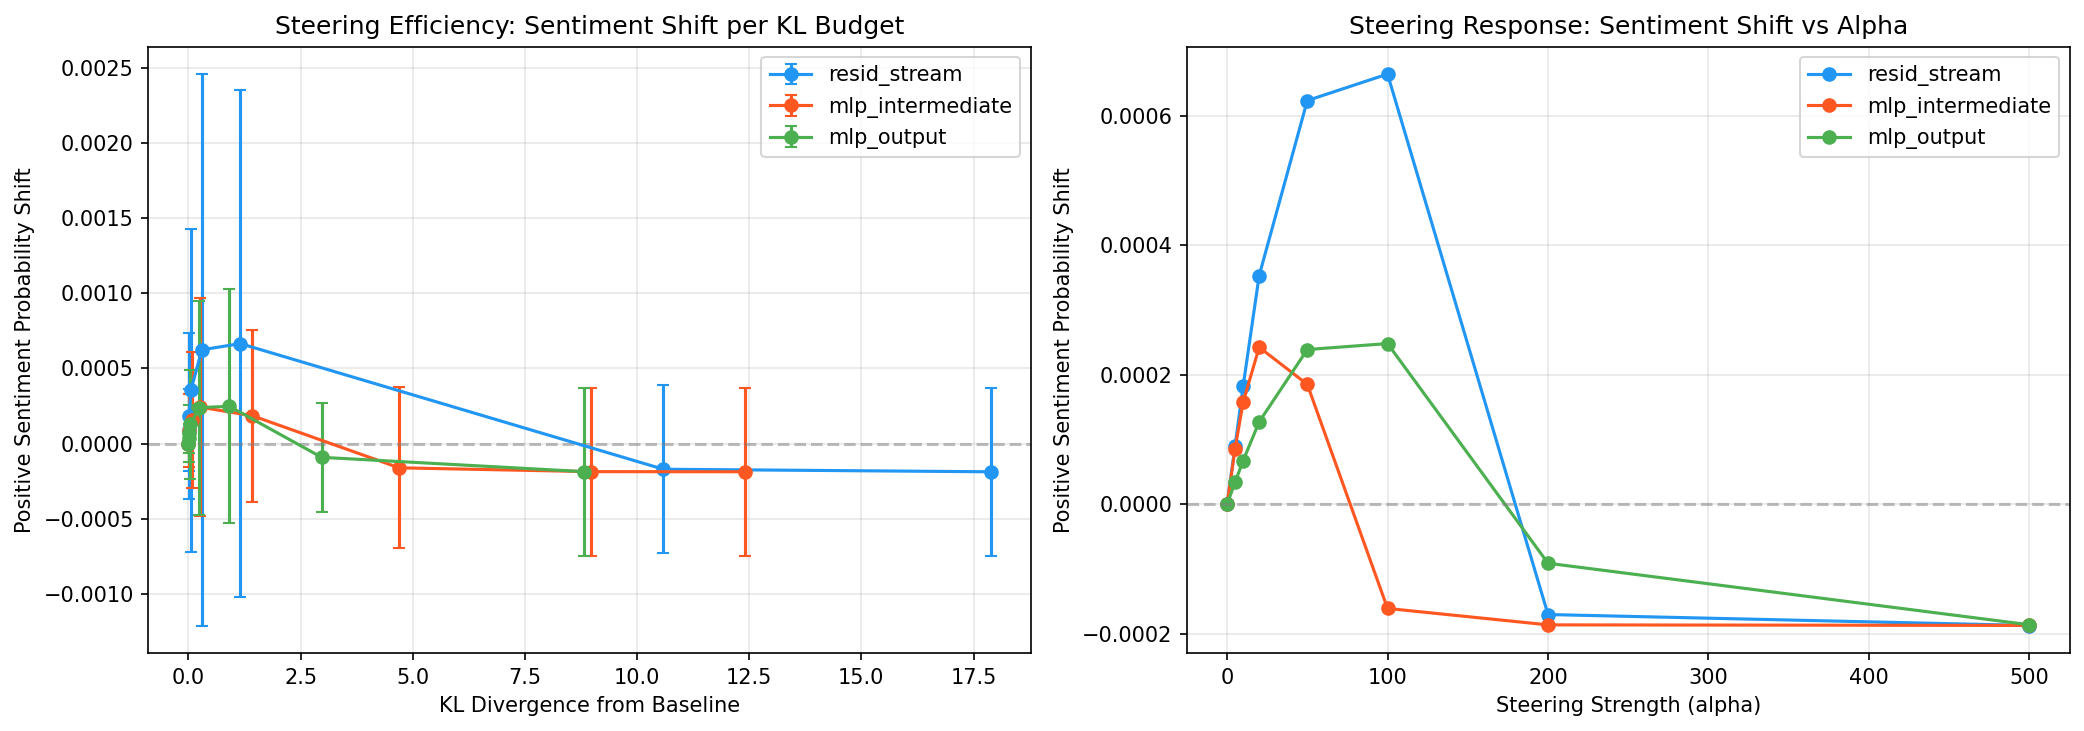
\includegraphics[width=0.95\linewidth]{figures/enhanced_steering_efficiency.png}
\caption{Steering efficiency as a function of intervention strength ($\alpha$). \figleft Sentiment probability shift. \figright Efficiency (shift per unit KL). The residual stream (blue) dominates at all operating points. All spaces show the characteristic inverted-U pattern, with the MLP intermediate space (green) peaking earlier and at a lower magnitude.}
\label{fig:efficiency}
\end{figure}

\subsection{Linear Separability}
\label{sec:linearity}

\Tabref{tab:probes} reports 5-fold cross-validated linear probe accuracy for sentiment classification at layer 8. Despite its $4\times$ higher dimensionality, the MLP intermediate space is \emph{less} linearly separable than the residual stream (76.0\% vs.\ 86.0\%), with higher variance across folds.

\begin{table}[t]
\centering
\caption{Linear probe accuracy (5-fold CV) for sentiment classification at layer 8. The residual stream achieves the highest accuracy despite having the fewest dimensions. Higher dimensionality does not imply greater linear separability.}
\label{tab:probes}
\begin{tabular}{@{}lcc@{}}
\toprule
Space & Dimensionality & Accuracy \\
\midrule
\residstream & 768 & {\bf 0.860 $\pm$ 0.102} \\
\mlpout & 768 & 0.800 $\pm$ 0.063 \\
\mlpinter & 3072 & 0.760 $\pm$ 0.163 \\
\bottomrule
\end{tabular}
\end{table}

\para{Multi-layer analysis.}
\Tabref{tab:layers} confirms this pattern across layers 6--10. The residual stream is more separable than the MLP intermediate space in 4 of 5 layers, with the gap widening in later layers (layer 10: 80.0\% vs.\ 70.0\%). The sole exception is layer 6, where the MLP intermediate space slightly leads (84.0\% vs.\ 82.0\%)---possibly because early-layer MLP representations are more distributed and less specialized.

\begin{table}[t]
\centering
\caption{Linear probe accuracy across layers 6--10. The residual stream advantage is consistent and grows in later layers, where MLP neurons become increasingly specialized.}
\label{tab:layers}
\begin{tabular}{@{}lccc@{}}
\toprule
Layer & \residstream & \mlpinter & \mlpout \\
\midrule
6 & 0.820 & {\bf 0.840} & 0.780 \\
7 & {\bf 0.900} & 0.800 & 0.880 \\
8 & {\bf 0.860} & 0.760 & 0.800 \\
9 & {\bf 0.860} & 0.720 & 0.880 \\
10 & {\bf 0.800} & 0.700 & 0.820 \\
\bottomrule
\end{tabular}
\end{table}

\begin{figure}[t]
\centering
\begin{minipage}{0.48\textwidth}
    \centering
    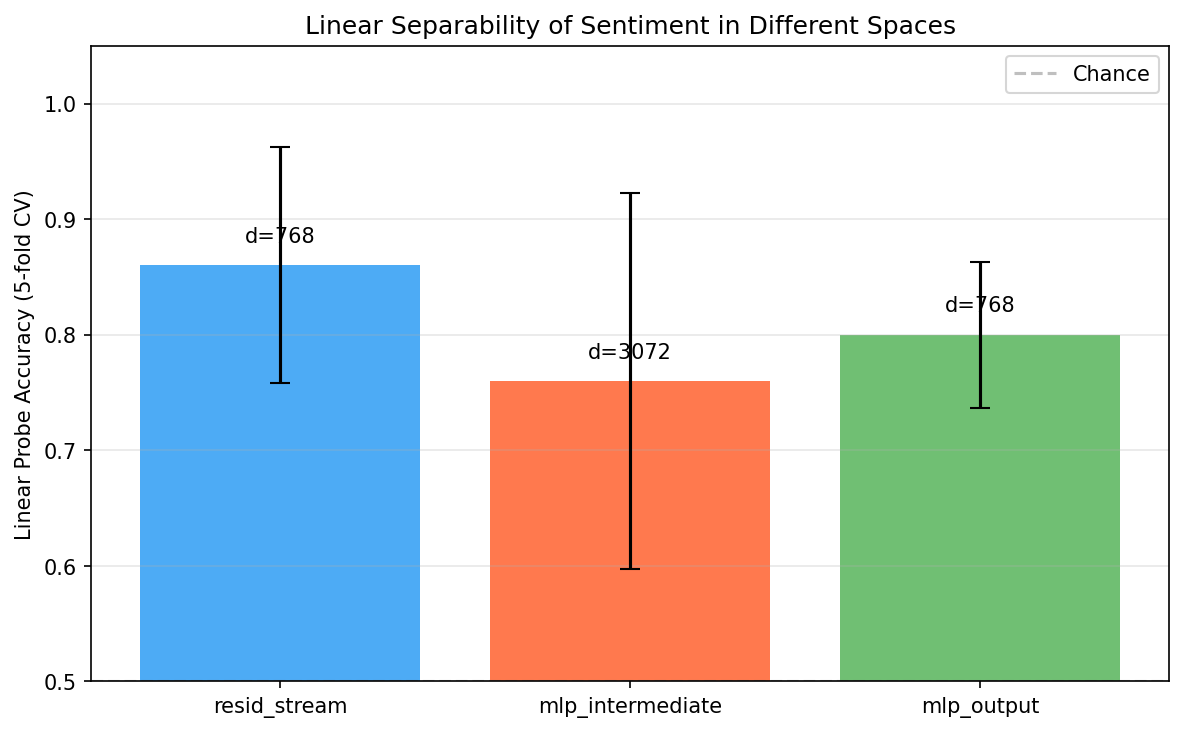
\includegraphics[width=\linewidth]{figures/linearity_comparison.png}
\end{minipage}
\hfill
\begin{minipage}{0.48\textwidth}
    \centering
    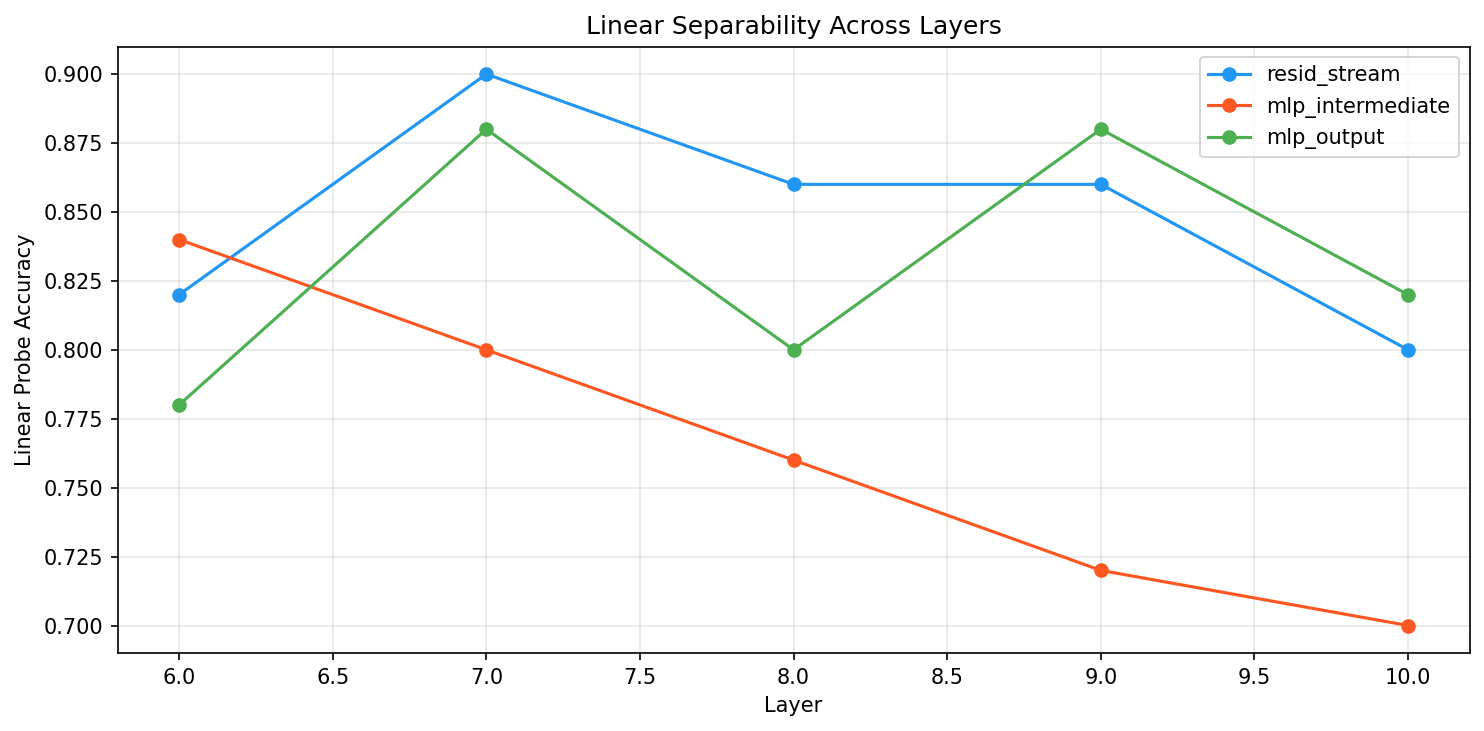
\includegraphics[width=\linewidth]{figures/layer_linearity.png}
\end{minipage}
\caption{\figleft Linear probe accuracy at layer 8 across spaces. \figright Probe accuracy across layers 6--10. The residual stream (blue) is consistently more separable, with the gap widening in later layers.}
\label{fig:linearity}
\end{figure}

\subsection{Sparsity Structure}
\label{sec:sparsity}

\para{Steering vector sparsity.}
The MLP intermediate steering vector is remarkably concentrated (\Tabref{tab:sv_sparsity}). Just 86 neurons (2.8\% of 3072) account for 50\% of the squared norm, and 609 neurons (19.8\%) account for 90\%. The single most important neuron (index 2002) contributes 4.4\% of the steering signal alone. By contrast, the residual stream steering vector requires 43.0\% of its dimensions for 90\% of the norm---it is far more distributed.

\begin{table}[t]
\centering
\caption{Steering vector concentration. The MLP intermediate steering vector is highly sparse: 2.8\% of neurons carry 50\% of the signal, compared to 43\% of dimensions in the residual stream.}
\label{tab:sv_sparsity}
\begin{tabular}{@{}lccc@{}}
\toprule
Metric & \residstream & \mlpinter & \mlpout \\
\midrule
Dims for 50\% norm$^2$ & --- & {\bf 86 (2.8\%)} & --- \\
Dims for 90\% norm$^2$ & 330 (43.0\%) & {\bf 609 (19.8\%)} & 336 (43.8\%) \\
Dims for 99\% norm$^2$ & --- & 1648 (53.6\%) & --- \\
Normalized entropy & 0.954 & {\bf 0.923} & 0.955 \\
SV sparsity (zero frac.) & 5.2\% & {\bf 23.1\%} & 3.4\% \\
\bottomrule
\end{tabular}
\end{table}

\begin{figure}[t]
\centering
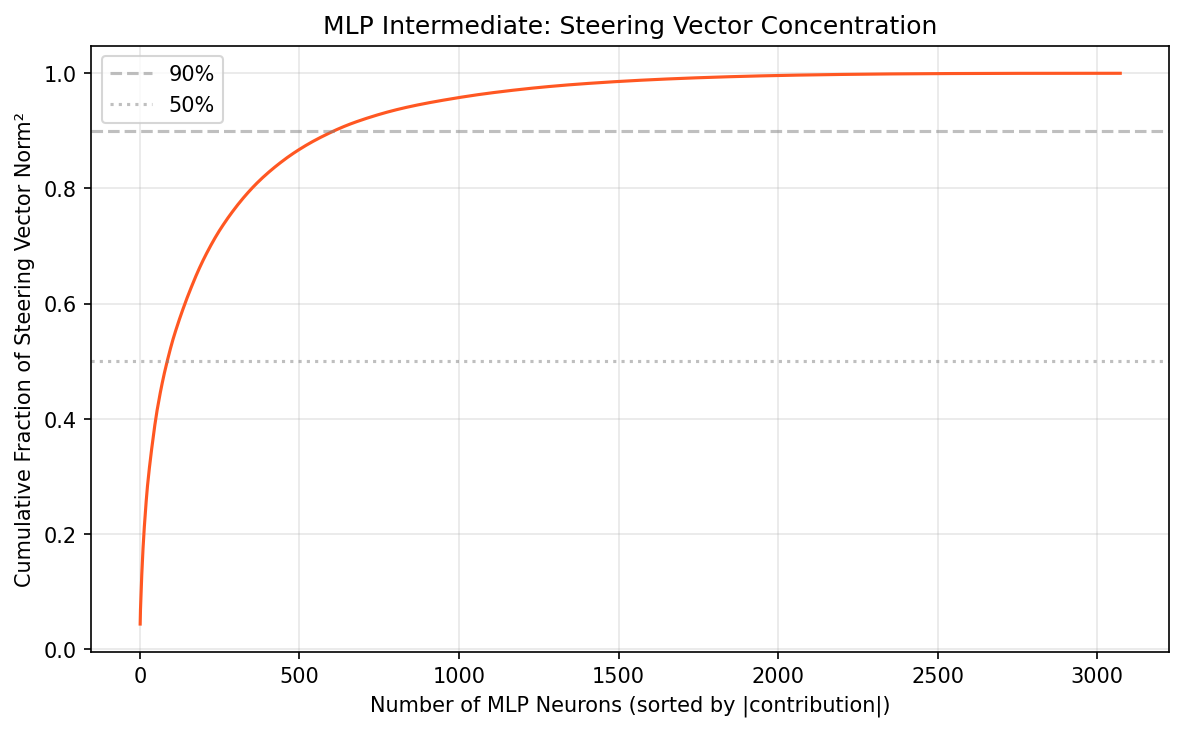
\includegraphics[width=0.6\linewidth]{figures/mlp_sv_concentration.png}
\caption{Cumulative squared norm of the MLP intermediate steering vector as a function of the number of neurons (sorted by magnitude). The curve rises steeply: 86 neurons (2.8\%) capture 50\% of the signal, and the top 609 (19.8\%) capture 90\%.}
\label{fig:sv_concentration}
\end{figure}

\para{Activation sparsity.}
Counterintuitively, MLP intermediate \emph{activations} are not sparser than residual stream activations by Gini coefficient (\Tabref{tab:act_sparsity}). The residual stream has a higher Gini coefficient (0.443 vs.\ 0.223), meaning its activations are more concentrated. However, the MLP intermediate space has substantially higher kurtosis (9.5 vs.\ 5.4), indicating heavier tails---a few neurons activate very strongly while most remain near their mean. This pattern is consistent with a space containing both many low-level active neurons and a few highly active ``expert'' neurons.

\begin{table}[t]
\centering
\caption{Activation sparsity metrics. The MLP intermediate space has lower Gini coefficient (less sparse overall) but higher kurtosis (more extreme outliers), consistent with a small number of expert neurons amid many weakly active ones.}
\label{tab:act_sparsity}
\begin{tabular}{@{}lccc@{}}
\toprule
Metric & \residstream & \mlpinter & \mlpout \\
\midrule
$L^0$ (near-zero frac.) & {\bf 0.382} & 0.108 & 0.330 \\
Gini coefficient & {\bf 0.443} & 0.223 & 0.329 \\
Kurtosis & 5.4 & {\bf 9.5} & 6.6 \\
Top-10\% concentration & {\bf 0.365} & 0.194 & 0.281 \\
\bottomrule
\end{tabular}
\end{table}

\subsection{Cross-Space Alignment}
\label{sec:alignment}

To understand how the steering vectors relate across spaces, we project the MLP intermediate vector through the down-projection matrix $\mW_{\text{out}}$ and compute cosine similarities (\Tabref{tab:alignment}).

\begin{table}[t]
\centering
\caption{Cosine similarity between steering vectors across spaces. The projected MLP intermediate vector and the MLP output vector are identical (cosine similarity 1.000), validating the methodology. The moderate alignment with the residual stream (0.474) indicates the vectors capture related but distinct aspects of sentiment.}
\label{tab:alignment}
\begin{tabular}{@{}lc@{}}
\toprule
Comparison & Cosine Similarity \\
\midrule
\residstream vs.\ projected(\mlpinter) & 0.474 \\
\residstream vs.\ \mlpout & 0.474 \\
projected(\mlpinter) vs.\ \mlpout & {\bf 1.000} \\
\bottomrule
\end{tabular}
\end{table}

The perfect cosine similarity between the projected MLP intermediate vector and the MLP output vector is expected---the MLP output is exactly $\mW_{\text{out}}$ applied to the intermediate activations. The moderate alignment (0.474) between the residual stream vector and the MLP-derived vectors reflects the fact that the residual stream integrates contributions from both attention and MLP, while the MLP vectors capture only the MLP's contribution to sentiment.

\subsection{Qualitative Steering Examples}
\label{sec:qualitative}

\Tabref{tab:examples} shows steered generations for the neutral prompt ``The weather today is'' at varying $\alpha$ values. Both spaces produce coherent, positively-steered text at moderate $\alpha$. At high $\alpha$, both degenerate---but the MLP intermediate space breaks down at lower $\alpha$ values and in a qualitatively different way (repeating numeric tokens vs.\ repeating characters).

\begin{table}[t]
\centering
\caption{Steered generations for ``The weather today is\ldots'' at different $\alpha$ values. The MLP intermediate space produces coherent positive text at moderate $\alpha$ but degrades to repetitive tokens at lower intervention strengths than the residual stream.}
\label{tab:examples}
\resizebox{\textwidth}{!}{
\begin{tabular}{@{}llp{8.5cm}@{}}
\toprule
Space & $\alpha$ & Continuation \\
\midrule
\residstream & 50 & ``\ldots is good for a good time in the United States.'' \\
\mlpinter & 50 & ``\ldots is a great day to visit. The day is to be a great day to visit.'' \\
\midrule
\residstream & 200 & ``\ldots isAAAAAAAAAAAAAAAAAAAAAAAAAAAAAA'' \\
\mlpinter & 200 & ``\ldots is191919191919191919191919191919'' \\
\bottomrule
\end{tabular}
}
\end{table}

\subsection{Hypothesis Summary}
\label{sec:hypotheses}

\Tabref{tab:hypotheses} summarizes the status of our four hypotheses.

\begin{table}[t]
\centering
\caption{Summary of hypothesis testing results.}
\label{tab:hypotheses}
\begin{tabular}{@{}lll@{}}
\toprule
Hypothesis & Result & Key Evidence \\
\midrule
H1: MLP steering produces concept-aligned text & Supported & Positive $\Delta_{\text{sent}}$ at moderate $\alpha$ \\
H2: MLP space is more linearly separable & Rejected & Probe: 76\% vs.\ 86\% (residual) \\
H3: MLP space has concentrated concept info & Partial & 2.8\% neurons $\rightarrow$ 50\% signal \\
H4: MLP steering is more/less reliable & Inconclusive & Similar CV at matched KL \\
\bottomrule
\end{tabular}
\end{table}
